% Dealing the binary digits of one uniform number into infinitely many. Generated by a short script.
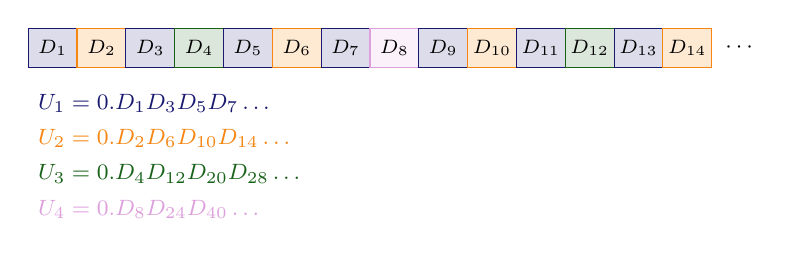
\begin{tikzpicture}
\draw[MidnightBlue,fill=MidnightBlue!15] (0.00,0) rectangle (0.62,0.5);
\node[font=\scriptsize] at (0.31,0.25) {$D_{1}$};
\draw[BurntOrange,fill=BurntOrange!15] (0.62,0) rectangle (1.24,0.5);
\node[font=\scriptsize] at (0.93,0.25) {$D_{2}$};
\draw[MidnightBlue,fill=MidnightBlue!15] (1.24,0) rectangle (1.86,0.5);
\node[font=\scriptsize] at (1.55,0.25) {$D_{3}$};
\draw[ForestGreen!70!black,fill=ForestGreen!70!black!15] (1.86,0) rectangle (2.48,0.5);
\node[font=\scriptsize] at (2.17,0.25) {$D_{4}$};
\draw[MidnightBlue,fill=MidnightBlue!15] (2.48,0) rectangle (3.10,0.5);
\node[font=\scriptsize] at (2.79,0.25) {$D_{5}$};
\draw[BurntOrange,fill=BurntOrange!15] (3.10,0) rectangle (3.72,0.5);
\node[font=\scriptsize] at (3.41,0.25) {$D_{6}$};
\draw[MidnightBlue,fill=MidnightBlue!15] (3.72,0) rectangle (4.34,0.5);
\node[font=\scriptsize] at (4.03,0.25) {$D_{7}$};
\draw[Plum,fill=Plum!15] (4.34,0) rectangle (4.96,0.5);
\node[font=\scriptsize] at (4.65,0.25) {$D_{8}$};
\draw[MidnightBlue,fill=MidnightBlue!15] (4.96,0) rectangle (5.58,0.5);
\node[font=\scriptsize] at (5.27,0.25) {$D_{9}$};
\draw[BurntOrange,fill=BurntOrange!15] (5.58,0) rectangle (6.20,0.5);
\node[font=\scriptsize] at (5.89,0.25) {$D_{10}$};
\draw[MidnightBlue,fill=MidnightBlue!15] (6.20,0) rectangle (6.82,0.5);
\node[font=\scriptsize] at (6.51,0.25) {$D_{11}$};
\draw[ForestGreen!70!black,fill=ForestGreen!70!black!15] (6.82,0) rectangle (7.44,0.5);
\node[font=\scriptsize] at (7.13,0.25) {$D_{12}$};
\draw[MidnightBlue,fill=MidnightBlue!15] (7.44,0) rectangle (8.06,0.5);
\node[font=\scriptsize] at (7.75,0.25) {$D_{13}$};
\draw[BurntOrange,fill=BurntOrange!15] (8.06,0) rectangle (8.68,0.5);
\node[font=\scriptsize] at (8.37,0.25) {$D_{14}$};
\node[font=\footnotesize,right] at (8.73,0.25) {$\cdots$};
\node[MidnightBlue,font=\footnotesize,anchor=west] at (0,-0.45) {$U_1=0.D_1D_3D_5D_7\ldots$};
\node[BurntOrange,font=\footnotesize,anchor=west] at (0,-0.90) {$U_2=0.D_2D_6D_{10}D_{14}\ldots$};
\node[ForestGreen!70!black,font=\footnotesize,anchor=west] at (0,-1.35) {$U_3=0.D_4D_{12}D_{20}D_{28}\ldots$};
\node[Plum,font=\footnotesize,anchor=west] at (0,-1.80) {$U_4=0.D_8D_{24}D_{40}\ldots$};
\end{tikzpicture}
